\section{Part 3: Examination of ERD and ERS}

\begin{taskbox}[Part 3: introduction in the lab manual]
The file \texttt{FiveClass\_EEG.mat} contains an EEG signal recorded at a sampling frequency of 256 Hz from one user while performing different mental tasks, from 30 channels of the international 10-20 system. Five mental tasks were assigned: (1) word generation, (2) mental subtraction, (3) navigation, (4) hand movement imagery and (5) foot movement imagery. In each trial, a ``+'' sign is first shown (time zero), after 3 seconds a beep is played and the task is shown, and the person performs the task for 7 seconds (until the second beep); between two trials there is a rest of 2.5 to 3.5 seconds. The data contain the matrix \texttt{X} (the recorded EEG), the vector \texttt{y} (the class label of each of the 200 trials) and the vector \texttt{trial} (the sample number of the start of each trial). We want to examine the changes of the signal in different frequency bands in each of the five classes.
\end{taskbox}

\subsection*{Data and task timing}

The continuous data of this part have 714701 samples and 30 channels and were recorded at a rate of 256~Hz. The 200 repetitions are divided into five classes, and each class has 40 repetitions: word generation, mental subtraction, navigation, hand movement imagery and foot movement imagery. Time zero is the display of the concentration cross; the task starts at about the third second and ends at the tenth second. The central channel CPz was chosen for the comparison plots.

\subsection*{(a) Four-band filtering}
\begin{taskbox}
First, filter the signal of each channel in the following four bands: delta (1 to 4 Hz), theta (4 to 8 Hz), alpha (8 to 13 Hz) and beta (13 to 30 Hz). For this purpose you can use the filter given in the manual (a 4th-order Chebyshev type I band-pass filter with 1 dB passband ripple, applied with \texttt{filter}). To make sure the filters work correctly, plot about 5 seconds of the first channel of \texttt{X}, the original signal and the four signals obtained in the different bands.
\end{taskbox}

The continuous signal of each channel was filtered with a type I Chebyshev filter of final order four and a ripple of one decibel. The filter was applied causally, as in the \texttt{filter} command of the experiment statement. In the SciPy implementation, an initial prototype order of two gives a final order of four after the band-pass transformation. The bands, according to the lab manual, are delta 1 to 4, theta 4 to 8, alpha 8 to 13 and beta 13 to 30~Hz.

\begin{figure}[H]
\centering
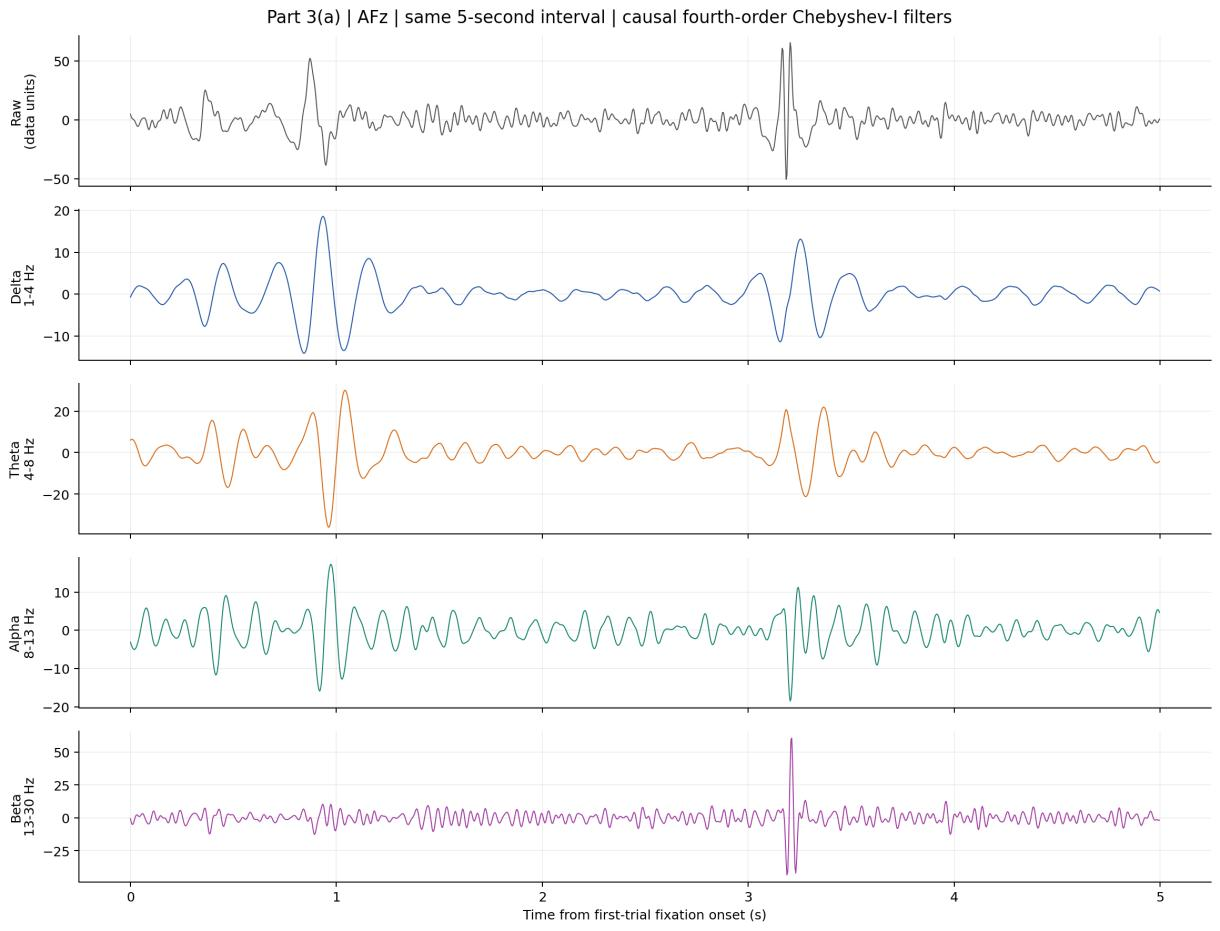
\includegraphics[width=0.9\textwidth]{fig09_erd_filter_check_afz.png}
\caption{The first five seconds of the first repetition in channel AFz; the raw signal and the output of all four bands over the same time interval.}
\label{fig:erdfilter}
\end{figure}

\subsection*{(b) to (e) Computing and smoothing the power}

\paragraph{(b) Separating the ten-second repetitions.}
\begin{taskbox}
Extract the 10-second trials from the obtained signals (using the information in the vector \texttt{trial}).
\end{taskbox}
After converting the start index, exactly 2560 samples were taken from each repetition. The tensor of each band therefore has dimensions 2560 samples $\times$ 30 channels $\times$ 200 repetitions. The index range of the MATLAB code in the PDF creates 2561 samples because it includes both ends; in this analysis the length of 2560 samples explicitly requested in the output dimensions was respected.

\paragraph{(c) and (d) Squared amplitude and the mean of each class.}
\begin{taskbox}
\textbf{(c)} To compute the power at each point, compute the square of the amplitude of all time points for each trial in each band and each channel.\\
\textbf{(d)} According to the labels of the 200 trials (in the vector \texttt{y}), separate the data of the 5 different classes and, for each band, obtain the mean of each channel over the trials of that class. The output is four tensors of size $2560\times30\times5$ (\texttt{Delta\_X\_avg}, \texttt{Theta\_X\_avg}, \texttt{Alpha\_X\_avg}, \texttt{Beta\_X\_avg}), where 30 is the number of channels and 5 the number of classes.
\end{taskbox}
The amplitude of all samples, in each repetition and each channel, was first squared. Then, with the label $y$, the power of the repetitions of each class was averaged. The output of each band is a tensor of $2560\times30\times5$. This order preserves the power of oscillations that have no phase locking, and it is consistent with the method of the lecture notes.
\begin{align}
p_{i,b,c}[k]&=\bigl(x_{i,b,c}[k]\bigr)^{2}\\
P_{j,b,c}[k]&=\frac{1}{n_j}\sum_{i\in I_j}p_{i,b,c}[k];\qquad n_j=40
\end{align}
In the relation above, the set of the indices of the repetitions of each class is shown with a subscripted symbol. The number of members of this set is 40 in each of the five classes.

\paragraph{(e) Temporal smoothing.}
\begin{taskbox}
To smooth the variations in the average signals of part (d), filter the signal of each channel in each of the trials and in each band using a rectangular window defined as \texttt{newWin = ones(1,200)/sqrt(200)} and the \texttt{conv} command.
\end{taskbox}
A rectangular window was built exactly according to the problem statement, with 200 coefficients equal to one over the square root of 200. The sum of the coefficients is 14.142; its output is therefore 14.142 times the conventional moving average with coefficients of one over 200. This scale is stated on the axis of the power plots. The convolution was performed in the \texttt{same} mode so that the time axis remains ten seconds.
\begin{equation}
w[k]=\frac{1}{\sqrt{200}}\qquad\text{for } 0\le k<200
\end{equation}
This window is about 0.78~s long and is applied centered; the effect of a change can spread to about 0.39~s on either side of it. Zero-padding at the two ends creates an artificial drop; the edge regions are shaded in the plots and were not the basis for interpreting the task changes.

\paragraph{Complementary measurement relative to the baseline.} For a relative comparison, the mean smoothed power in the interval 0.5 to 2.5~s was taken as the baseline of each class and channel. The percentage change was summarized in the interval 3.5 to 9.5~s. In this way, the convolution edges and the transition at the task onset were avoided. The constant coefficient of the window cancels in the following ratio; a negative sign is ERD and a positive sign is ERS.
\begin{equation}
\mathrm{ERD/ERS}[k]=100\times\frac{P[k]-R}{R}
\end{equation}

\subsection*{(f) Delta and theta band power at CPz}
\begin{taskbox}
Choose one channel (preferably a channel from the central regions of the head, such as CPz) and plot the results of part (e) for it: for each frequency band, plot the time-averaged signal (over the 10-second interval) of all 5 classes in one figure (four figures in total, with 5 curves in each figure).
\end{taskbox}

In each figure, the smoothed mean-power curves of the five classes are shown. The dashed line is the beginning of the task at the third second. The blue region is the baseline interval of the relative analysis, and the gray regions show the two convolution edges.

\begin{figure}[H]
\centering
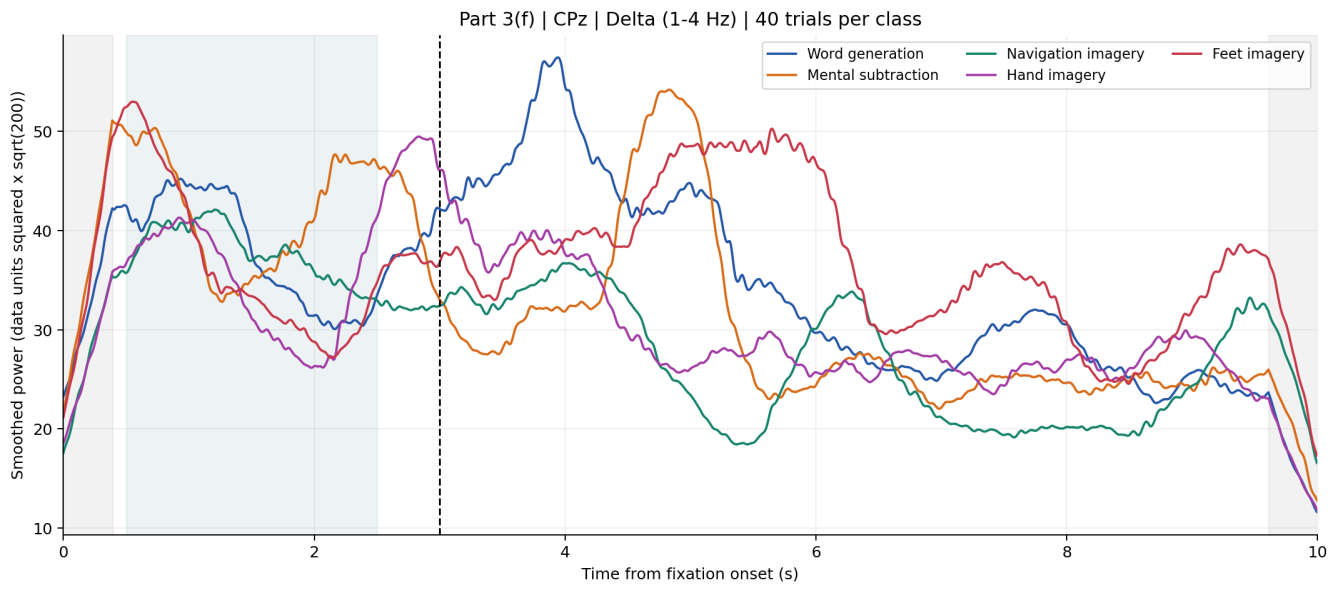
\includegraphics[width=0.85\textwidth]{fig10_delta_power_five_classes.png}
\caption{Smoothed delta power (1 to 4~Hz) in the five classes.}
\label{fig:delta}
\end{figure}

\begin{figure}[H]
\centering
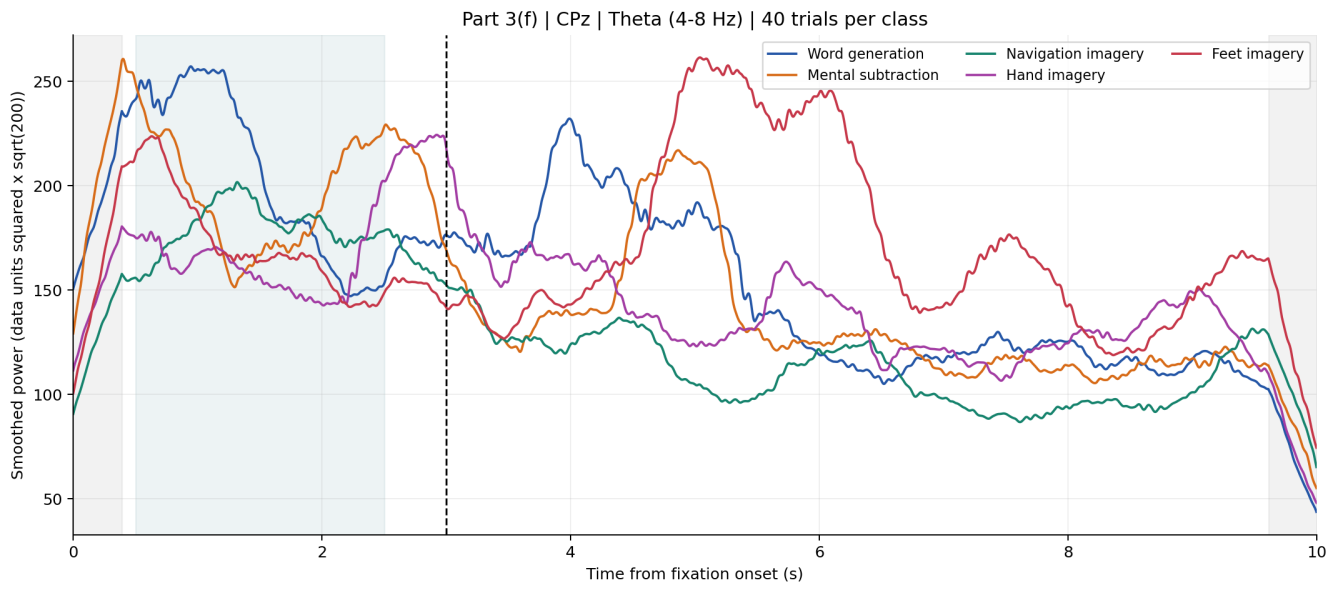
\includegraphics[width=0.85\textwidth]{fig11_theta_power_five_classes.png}
\caption{Smoothed theta power (4 to 8~Hz) in the five classes.}
\label{fig:theta}
\end{figure}

At CPz, navigation and subtraction show a decrease in delta and theta power over most of the activity interval. Foot imagery shows an increase in power in part of the interval. For comparing the classes, the difference in baseline power must also be taken into account; the size of the relative change cannot be concluded from the absolute height of the curves alone.

\subsection*{(f, continued) Alpha and beta band power at CPz}

\begin{figure}[H]
\centering
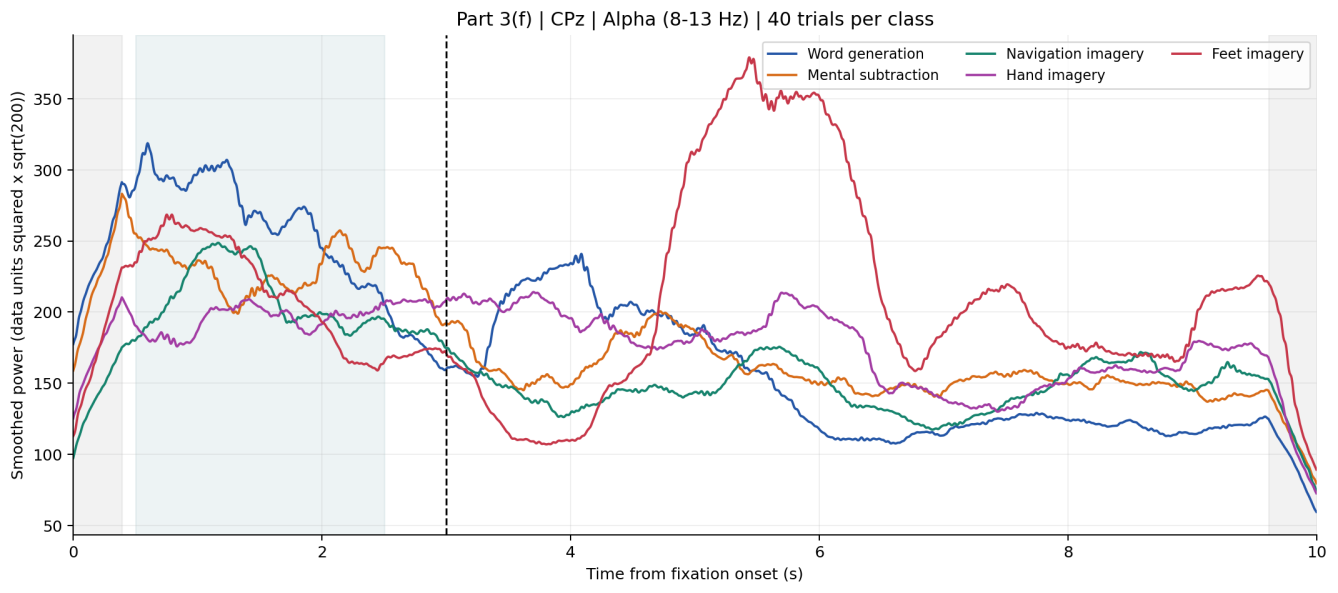
\includegraphics[width=0.85\textwidth]{fig12_alpha_power_five_classes.png}
\caption{Smoothed alpha power (8 to 13~Hz) in the five classes.}
\label{fig:alpha}
\end{figure}

\begin{figure}[H]
\centering
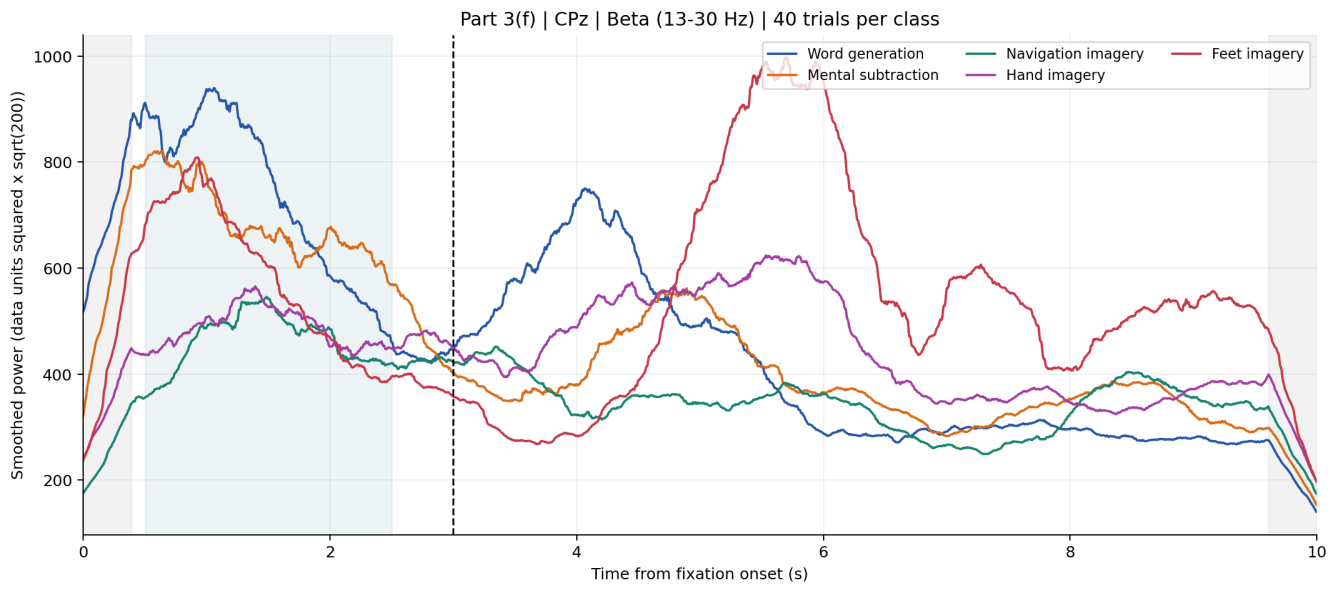
\includegraphics[width=0.85\textwidth]{fig13_beta_power_five_classes.png}
\caption{Smoothed beta power (13 to 30~Hz) in the five classes.}
\label{fig:beta}
\end{figure}

Word generation in this channel, especially in the second half of the task, shows a more definite decrease in alpha and beta. Foot imagery has a transient increase near the fifth and sixth seconds and then decreases; a single temporal average therefore does not reflect all the details of the trend. Hand imagery has smaller average changes than word generation and subtraction.

\subsection*{(g) Interpretation of the relative power changes}
\begin{taskbox}
Considering that the mental tasks start at approximately the third second, by comparing the plots obtained in part (f), what conclusions can be drawn about the frequency information of the five classes?
\end{taskbox}

\begin{table}[H]
\centering
\caption{Mean percentage change of the smoothed power at CPz during 3.5 to 9.5~s relative to the baseline of 0.5 to 2.5~s.}
\begin{tabular}{@{}lrrrr@{}}
\toprule
\textbf{Class} & \textbf{Delta (\%)} & \textbf{Theta (\%)} & \textbf{Alpha (\%)} & \textbf{Beta (\%)}\\
\midrule
Word generation & $-11.10$ & $-31.15$ & $-44.96$ & $-47.19$\\
Subtraction     & $-29.26$ & $-31.75$ & $-31.93$ & $-44.45$\\
Navigation      & $-32.06$ & $-39.87$ & $-30.93$ & $-27.53$\\
Hand imagery    & $-17.07$ & $-15.59$ & $-11.50$ & $-8.46$\\
Foot imagery    & $+3.18$  & $+1.81$  & $-1.86$  & $-4.53$\\
\bottomrule
\end{tabular}
\end{table}

\begin{figure}[H]
\centering
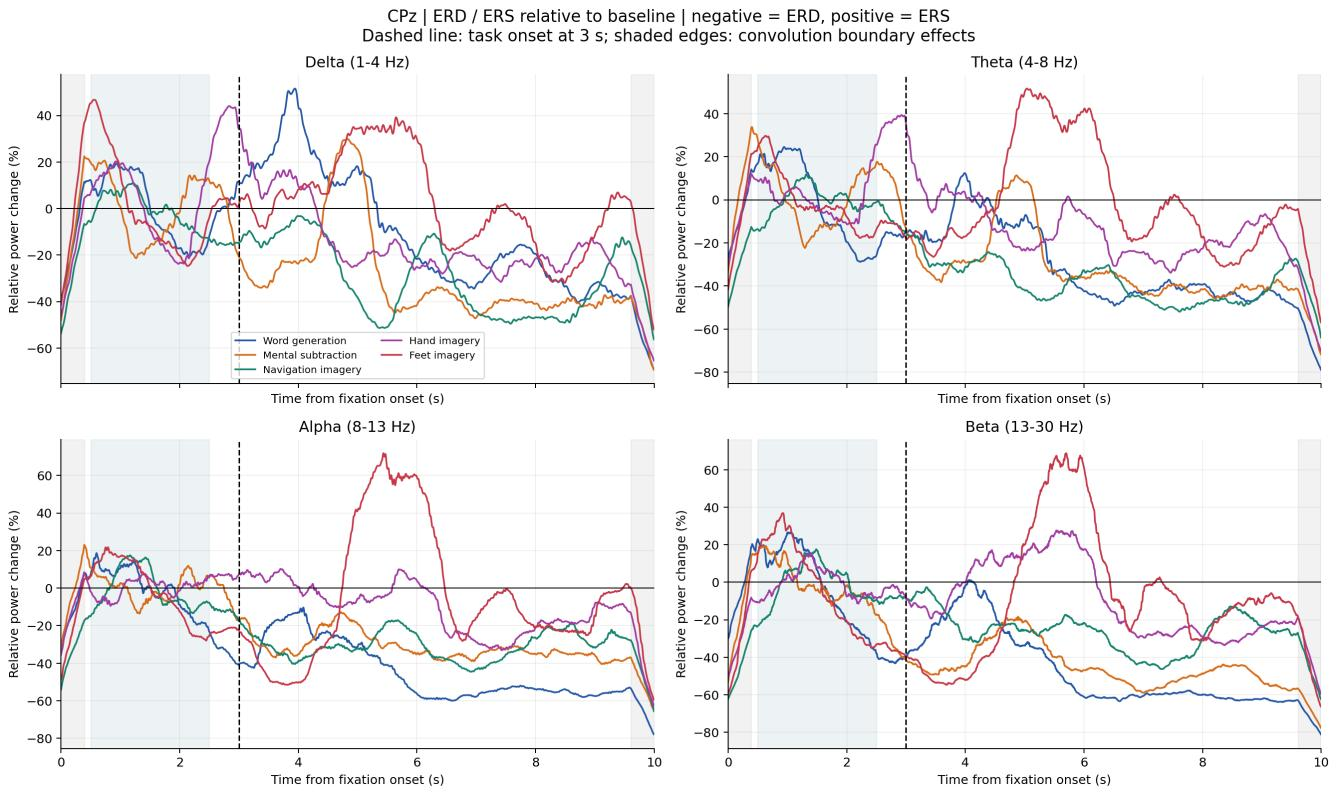
\includegraphics[width=0.85\textwidth]{fig14_relative_trend_four_bands.png}
\caption{Relative trend of the four bands; zero is the baseline power of the same class.}
\label{fig:relative}
\end{figure}

The largest average decrease of alpha and beta belongs to word generation, 44.96 and 47.19 percent, respectively, and the largest decrease of theta belongs to navigation, with 39.87 percent. Foot imagery has a smaller average change: delta and theta are slightly positive, and alpha and beta are slightly negative. This description is limited to channel CPz and the specified intervals and does not mean that there is no relevant activity in the other channels.

The difference between the class means can be a basis for extracting band-power features, but it does not prove the separability of the classes, statistical significance or classification accuracy. The readiness before the task, the delay of the causal filter and the centered smoothing also affect the interpretation of the time at which the changes begin.
